\chapter{Overview of the Past and Present Analyses}
\label{chap:History}

\ac{CLFV} search involving top quarks is an active area of research at the \ac{LHC} experiments. So far, no significant excess over the \ac{SM} predictions has been reported, and the observations from the \ac{ATLAS} and \ac{CMS} experiments are both interpreted using the framework of \ac{EFT}. Brief reviews of two past \ac{ATLAS} analyses and one past \ac{CMS} analysis are given in \autoref{sec:CLFV_ATLAS} and \autoref{sec:CLFV_CMS}, respectively. An overview of the present analysis is given in \autoref{sec:CLFV_This}.
%%%%%%%%%%%%%%%%%%%%%%%%%%%%%%%%%%%%%%%%%%%
%%%%%%%%%%%%%%%%%%%%%%%%%%%%%%%%%%%%%%%%%%%

\section{Past ATLAS Analyses}
\label{sec:CLFV_ATLAS}

The flavor-violating $\emut{q}$ interactions were first studied by the \ac{ATLAS} Collaboration~\cite{ATLAS-CONF-2018-044} using data collected during 2015-2017 at 13 TeV, corresponding to an integrated luminosity of 79.8 fb$^{-1}$. In addition to three leptons, this analysis targets final states with two or more jets. Only the top quark decay signal mode is considered. Lorentz structures of dimension-6 operators are not probed separately. Discriminating variables, such as the $\pt$ of the leptons, are combined into a \ac{BDT}, which is used to interpret the observation. A representative Feynman diagram targeted by this analysis and the distributions of the \ac{BDT} discriminator are shown in Figure~\ref{fig:ATLAS_results1}.

\begin{figure}[tbh!]
 \begin{center}
 \begin{minipage}[b]{0.325\linewidth} 
 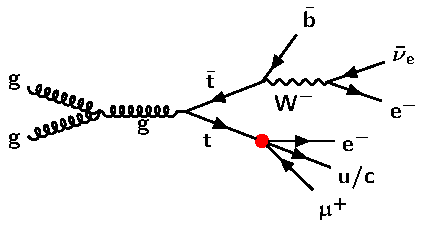
\includegraphics[width=\textwidth]{figures/Part3/History/TT} 
 \vspace{2em}
 \end{minipage}
 \hfill
 \begin{minipage}[b]{0.325\linewidth} 
 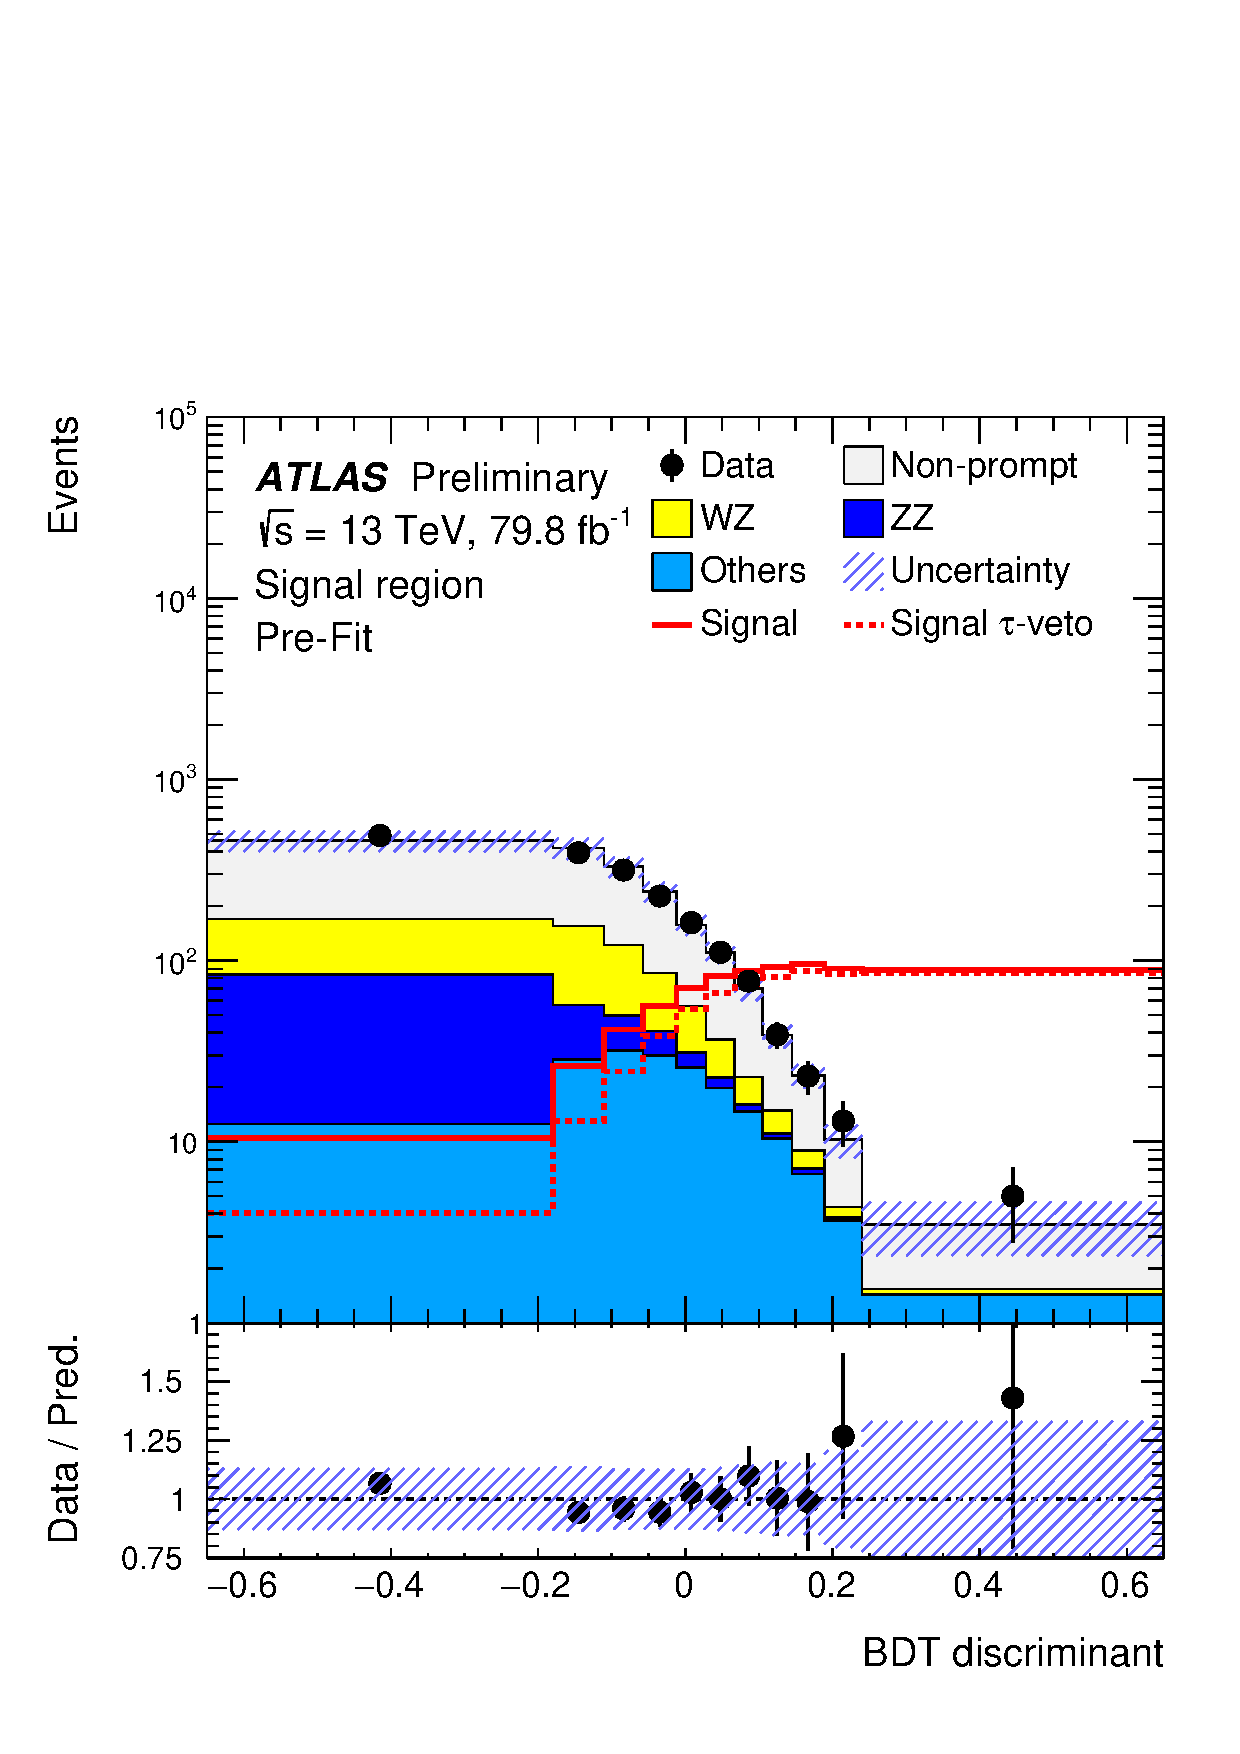
\includegraphics[width=\textwidth]{figures/Part3/History/ATLAS_results1}
 \end{minipage}
 \hfill
 \begin{minipage}[b]{0.325\linewidth} 
 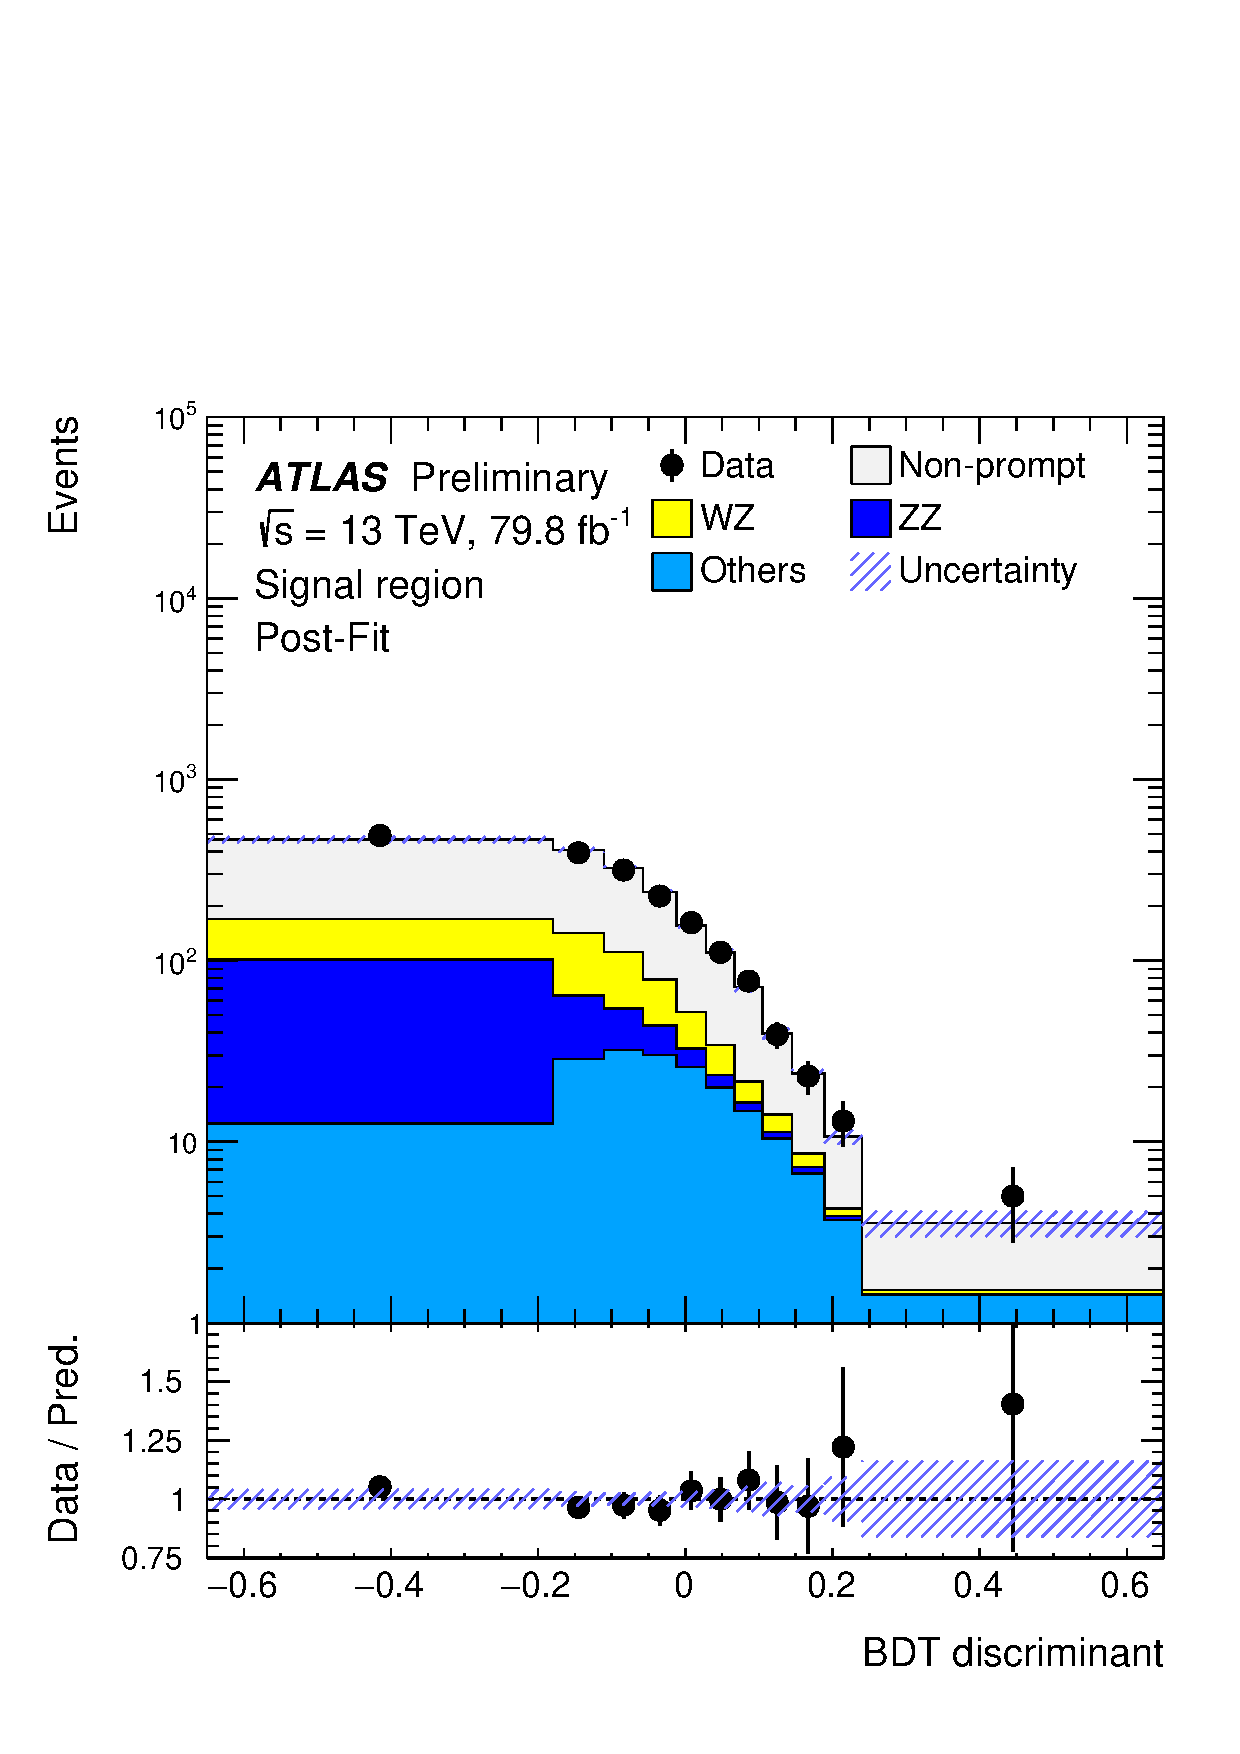
\includegraphics[width=\textwidth]{figures/Part3/History/ATLAS_results2}
 \end{minipage}
 \caption{Representative Feynman diagram for the \ac{CLFV} top quark decay processes that are targeted by \cite{ATLAS-CONF-2018-044} (left). The \ac{CLFV} interaction vertex is shown as a solid red circle to indicate that it is not allowed in the \ac{SM}. The middle (right) histogram shows the distribution of the pre-fit (post-fit) \ac{BDT} discriminator targeting the \ac{CLFV} top quark decay. }
 \label{fig:ATLAS_results1}
 \end{center}
\end{figure}

Data is found to be compatible with the \ac{SM} predictions, and an upper limit on the branching fraction of $\mathcal{B}(\tto{q}$) $<$ 6.6 $\times$ 10$^{-6}$ is set at 95\% \ac{CL}~\cite{Read2002}. This result improves a previous bound established in an indirect search~\cite{Davidson:2015zza} by three orders of magnitude. 

The \ac{ATLAS} Collaboration also studied the $\upmu\uptau$tq interactions 140 fb$^{-1}$ data collected in 2015-2018~\cite{ATLAS-CONF-2023-001}. This analysis targets final states with two \ac{SS} muons, one hadronic tau, and one or more jets. Both top quark production and decay signals are considered in this analysis. Operators with different Lorentz structures are considered separately. Representative Feynman diagrams are shown in Figure~\ref{fig:ATLAS_FD}. 

\begin{figure}[tbh!]
 \begin{center}
 \begin{tabular}{ccc}
 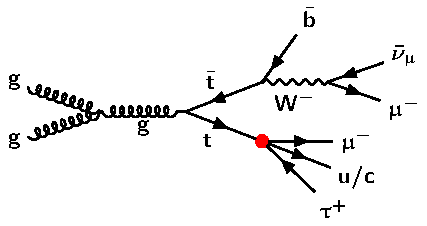
\includegraphics[width=0.31\textwidth]{figures/Part3/History/ATLAS_TT}&
 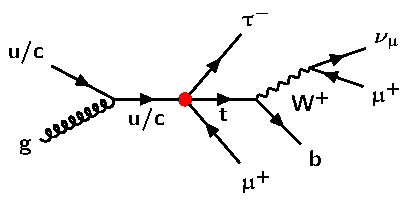
\includegraphics[width=0.33\textwidth]{figures/Part3/History/ATLAS_ST1}&
 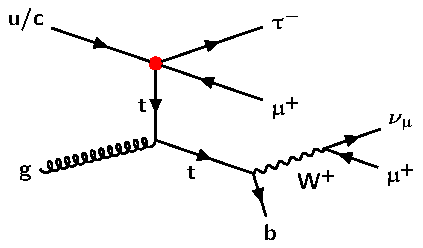
\includegraphics[width=0.31\textwidth]{figures/Part3/History/ATLAS_ST2}\\
 \end{tabular}
 \caption{Representative Feynman diagrams for the signal processes that are targeted by~\cite{ATLAS-CONF-2023-001}. Both top quark decay (left) and production (middle and right) \ac{CLFV} processes are shown. The two muons in the final states are required to have the same electric charge.}
 \label{fig:ATLAS_FD}
 \end{center}
\end{figure}

Due to limited statistics, event yields of the \acp{SR} are directly used to interpret the observation, which is shown in Figure~\ref{fig:ATLAS_results2}. An upper limit at 95\% \ac{CL} is placed on the branching fraction of $\mathcal{B}(\textsf{t}\rightarrow\upmu\uptau\textsf{q})$ $<$ 1.1 $\times$ 10$^{-6}$. The corresponding constraint on the \ac{WC} improves the previous bound~\cite{Chala:2018agk} by nearly a factor of 30.

\begin{figure}[tbh!]
 \begin{center}
 \begin{tabular}{cc}
 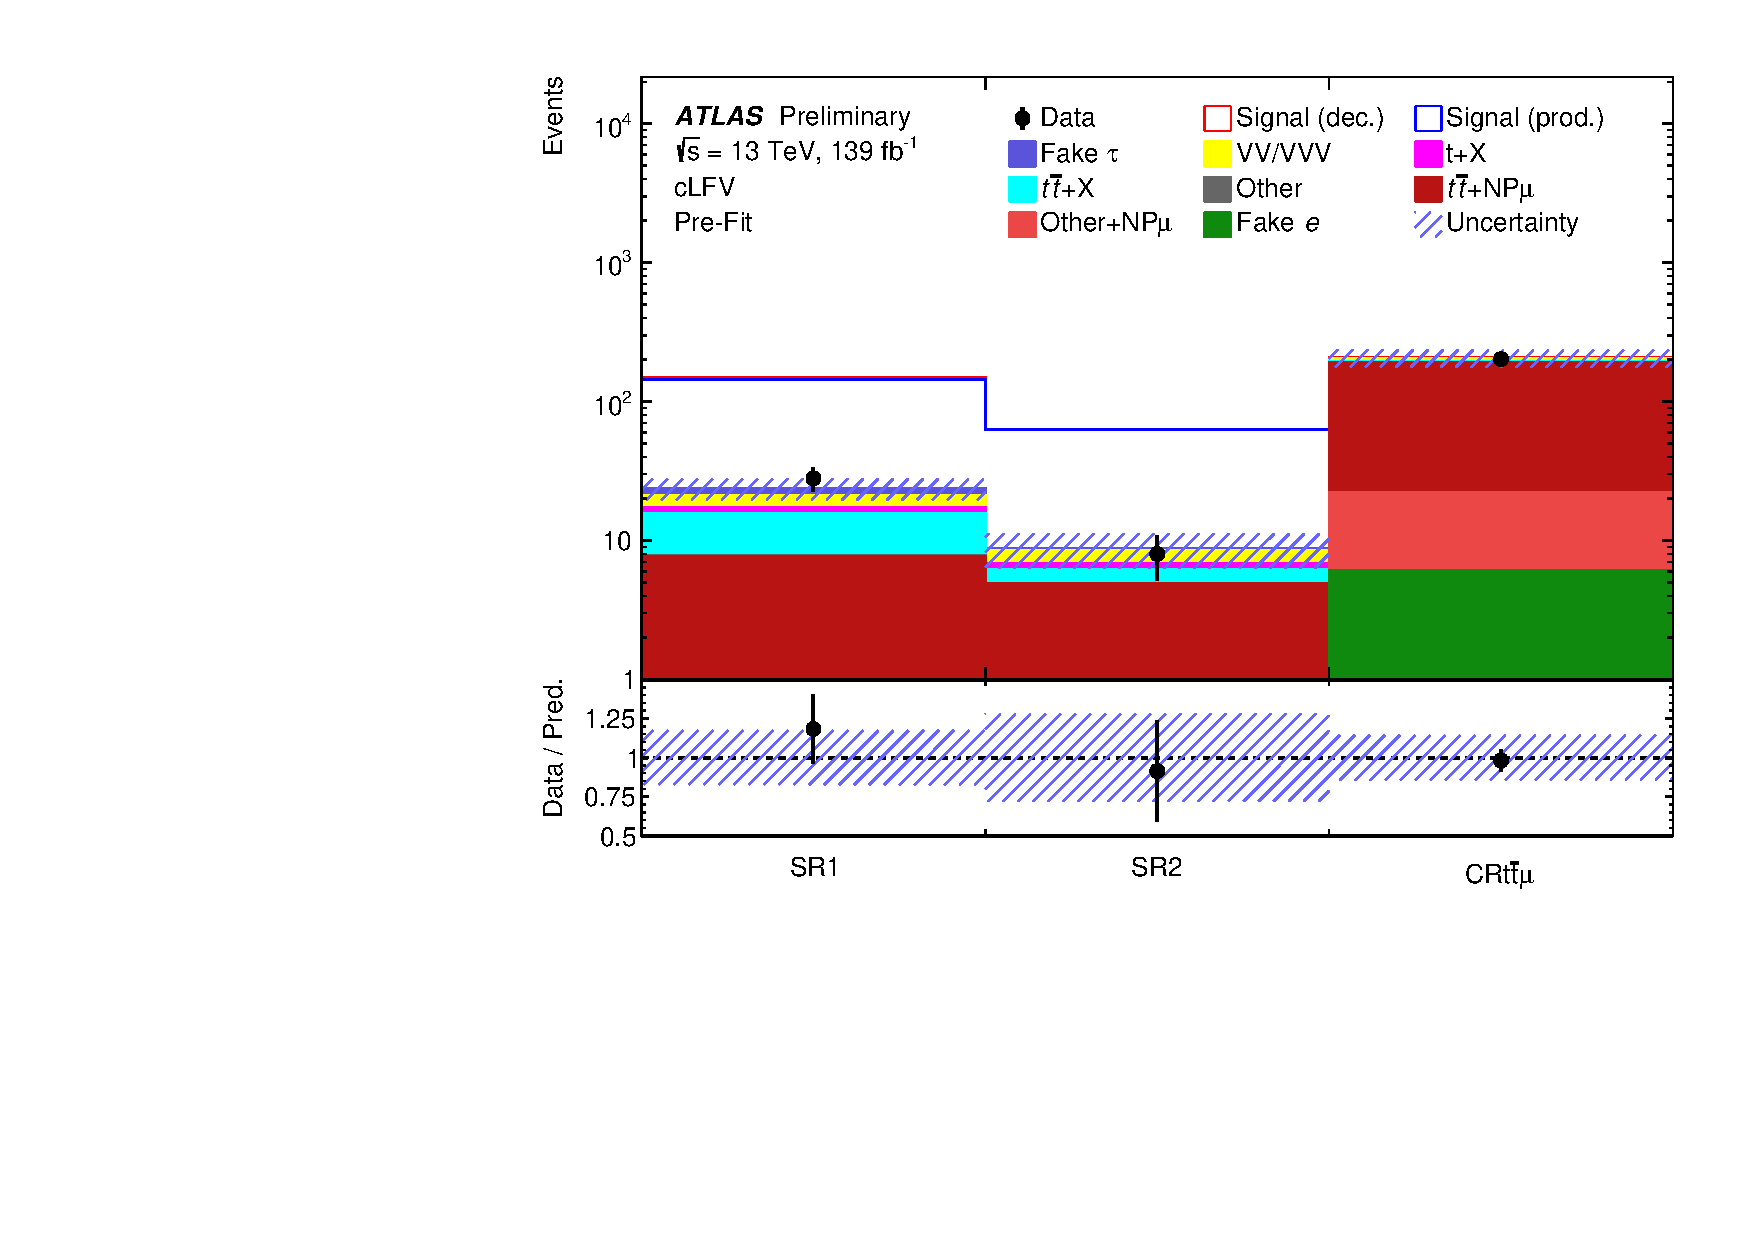
\includegraphics[width=0.48\textwidth]{figures/Part3/History/ATLAS_results3}&
 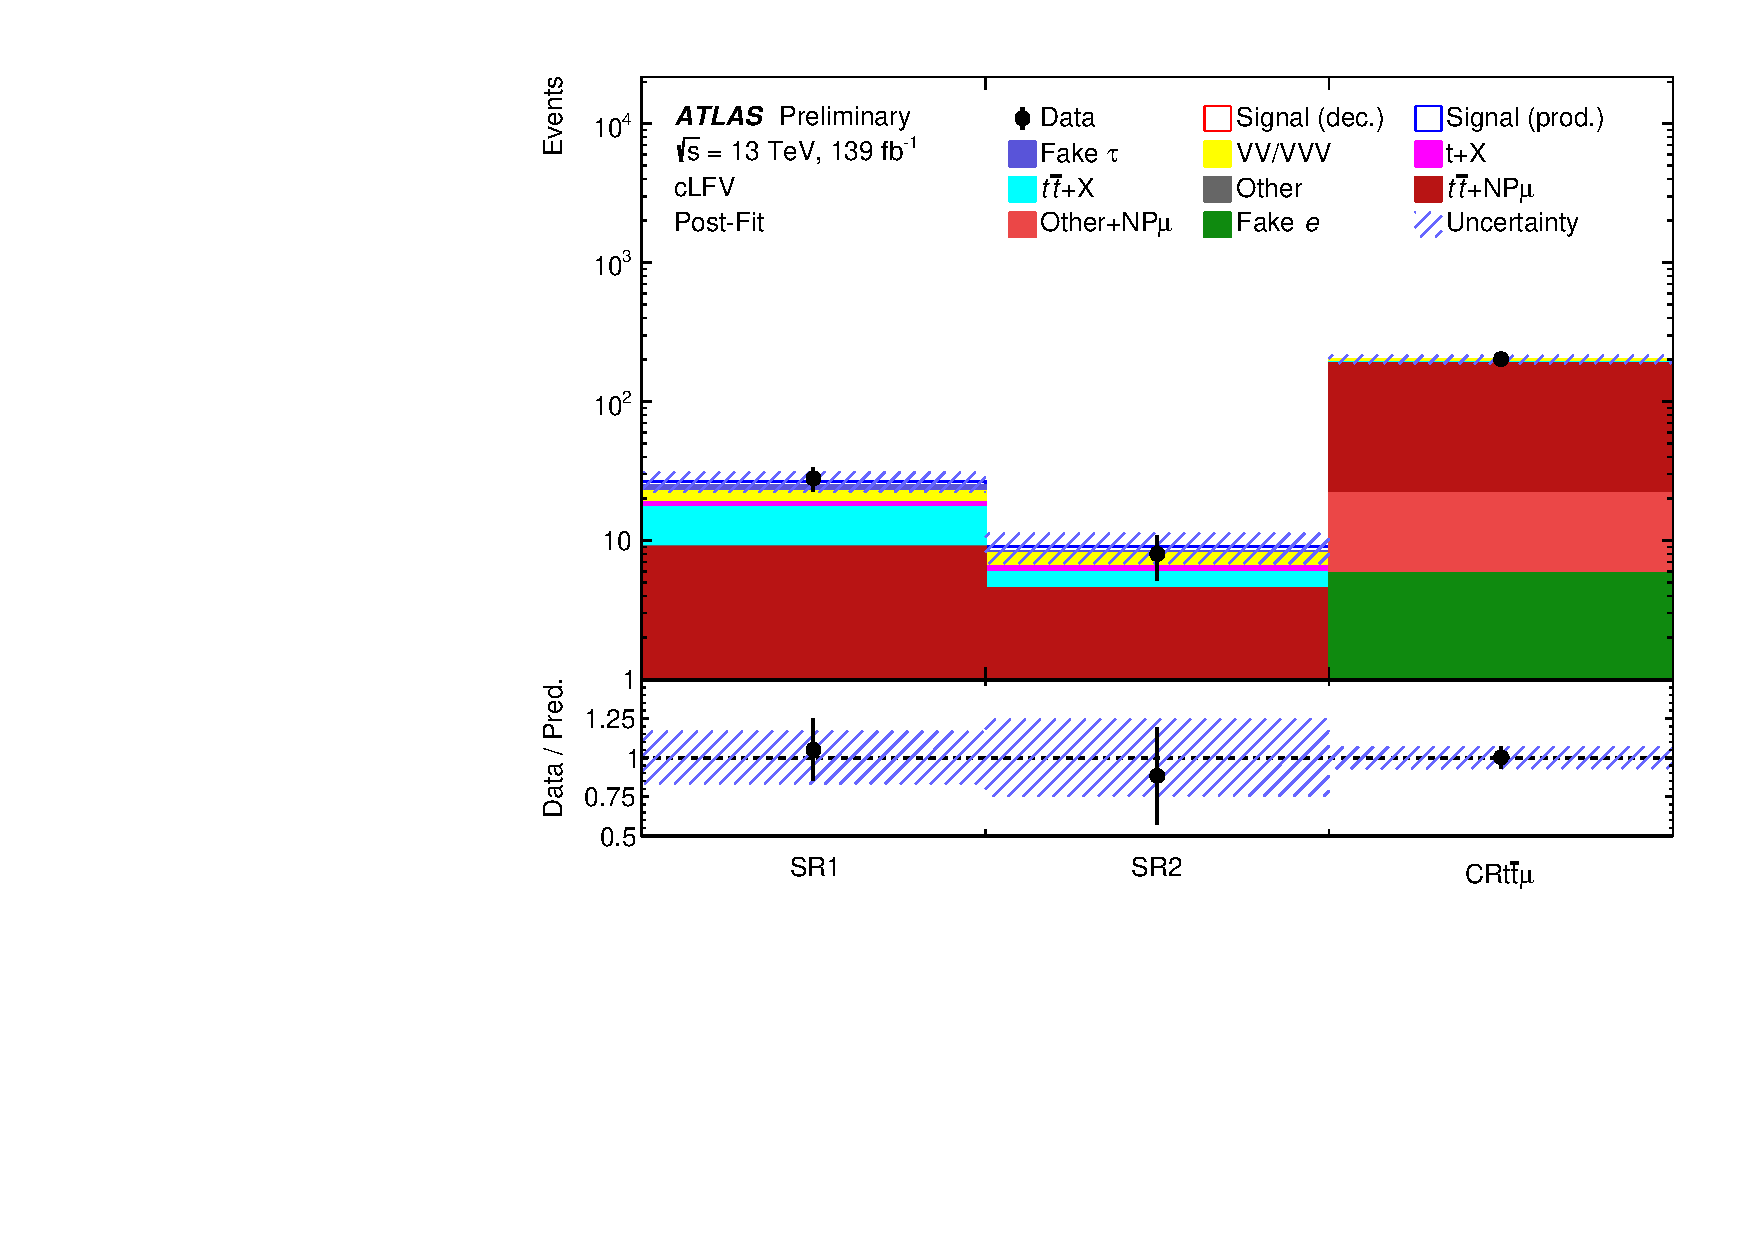
\includegraphics[width=0.48\textwidth]{figures/Part3/History/ATLAS_results4}\\
 \end{tabular}
 \caption{The left (right) histogram shows the pre-fit (post-fit) event yields of various regions studied by \cite{ATLAS-CONF-2023-001}. In these histograms, ``SR1'' denotes the signal region with two or more jets while ``SR2'' denotes the signal region with exactly one jet. ``CR$\ttbar\upmu$'' denotes the control region of the $\ttbar\upmu$ background, where the $\upmu$ is a \emph{nonprompt} muon.}
 \label{fig:ATLAS_results2}
 \end{center}
\end{figure}
%%%%%%%%%%%%%%%%%%%%%%%%%%%%%%%%%%%%%%%%%%%
%%%%%%%%%%%%%%%%%%%%%%%%%%%%%%%%%%%%%%%%%%%
\section{Past CMS Analysis}
\label{sec:CLFV_CMS}

The \ac{CMS} Collaboration followed up with a search for $\emut{q}$ interactions using data collected in 2016-2018~\cite{CMS:2022ztx}. Unlike the previous \ac{ATLAS} analysis~\cite{ATLAS-CONF-2018-044}, this \ac{CMS} analysis targets final states with two leptons and a hadronically decaying top quark. Both top quark production and decay signals are considered in this analysis. Operators with different Lorentz structures are considered separately. Representative Feynman diagrams are shown in Figure~\ref{fig:CMS_FD}. 

\begin{figure}[tbh!]
 \begin{center}
 \begin{tabular}{ccc}
 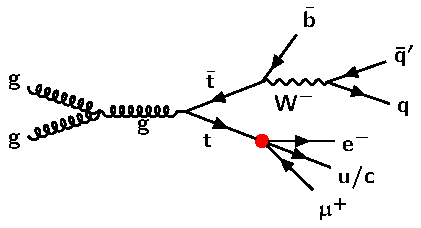
\includegraphics[width=0.31\textwidth]{figures/Part3/History/CMS_TT}&
 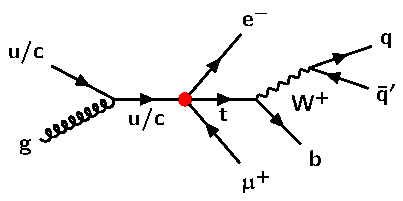
\includegraphics[width=0.33\textwidth]{figures/Part3/History/CMS_ST1}&
 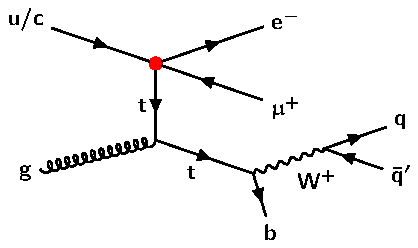
\includegraphics[width=0.31\textwidth]{figures/Part3/History/CMS_ST2}\\
 \end{tabular}
 \caption{Representative Feynman diagrams for the signal processes that are targeted by~\cite{CMS:2022ztx}. Both top quark decay (left) and production (middle and right) \ac{CLFV} processes are shown. The top quark that does not participate in the \ac{CLFV} interaction is required to produce fully hadronic final states.}
 \label{fig:CMS_FD}
 \end{center}
 \end{figure}
 
A \ac{BDT} using multiple discriminating variables is trained to further enhance the sensitivity. Distributions of the \ac{BDT} discriminator are shown in Figure~\ref{fig:CMS_results}. An upper limit at 95\% \ac{CL} is placed on the branching fraction of $\mathcal{B}(\textsf{t}\rightarrow\upmu\uptau\textsf{q})$ $<$ 7 $\times$ 10$^{-8}$, which improves the previous bound established by the \ac{ATLAS} Collaboration~\cite{ATLAS-CONF-2018-044} by two orders of magnitude.
 
 \begin{figure}[tbh!]
 \begin{center}
 \begin{tabular}{cc}
 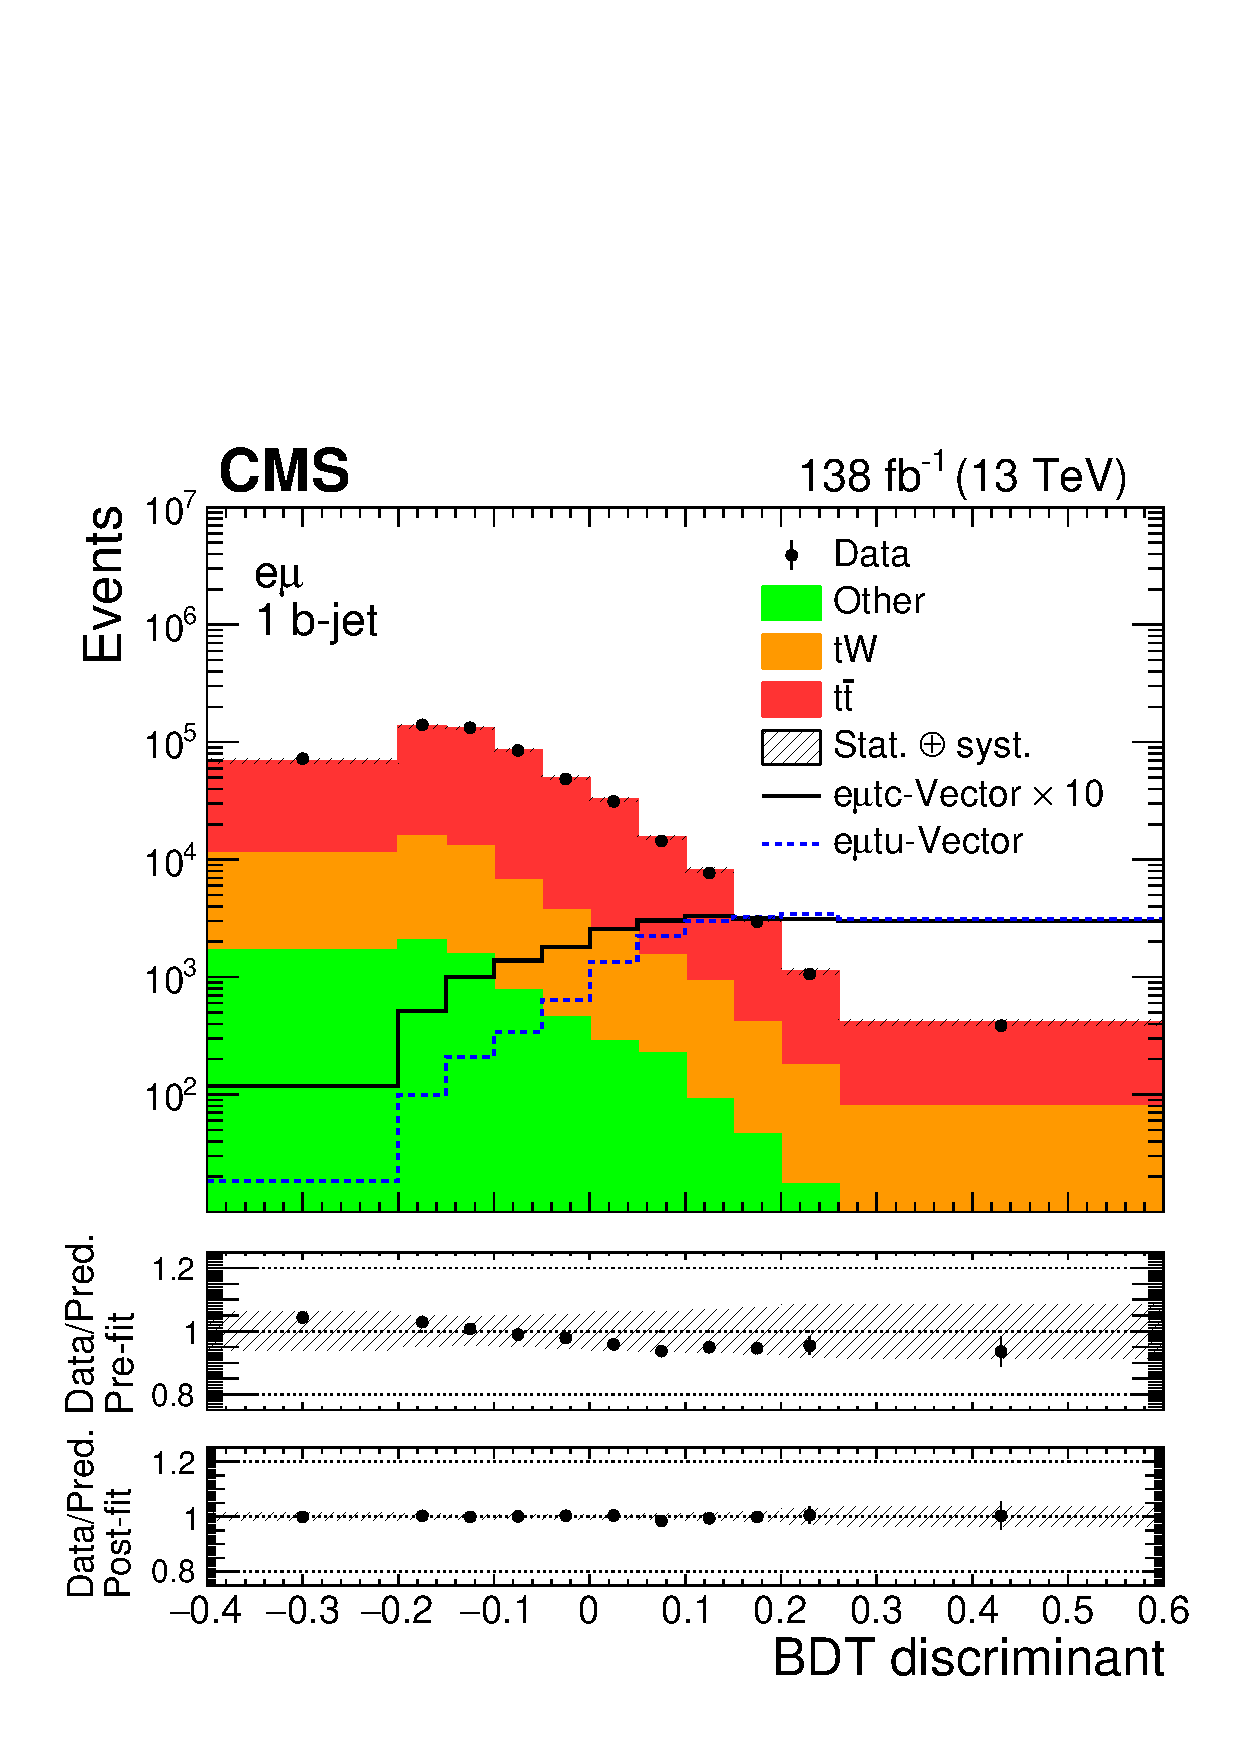
\includegraphics[width=0.48\textwidth]{figures/Part3/History/CMS_results1}&
 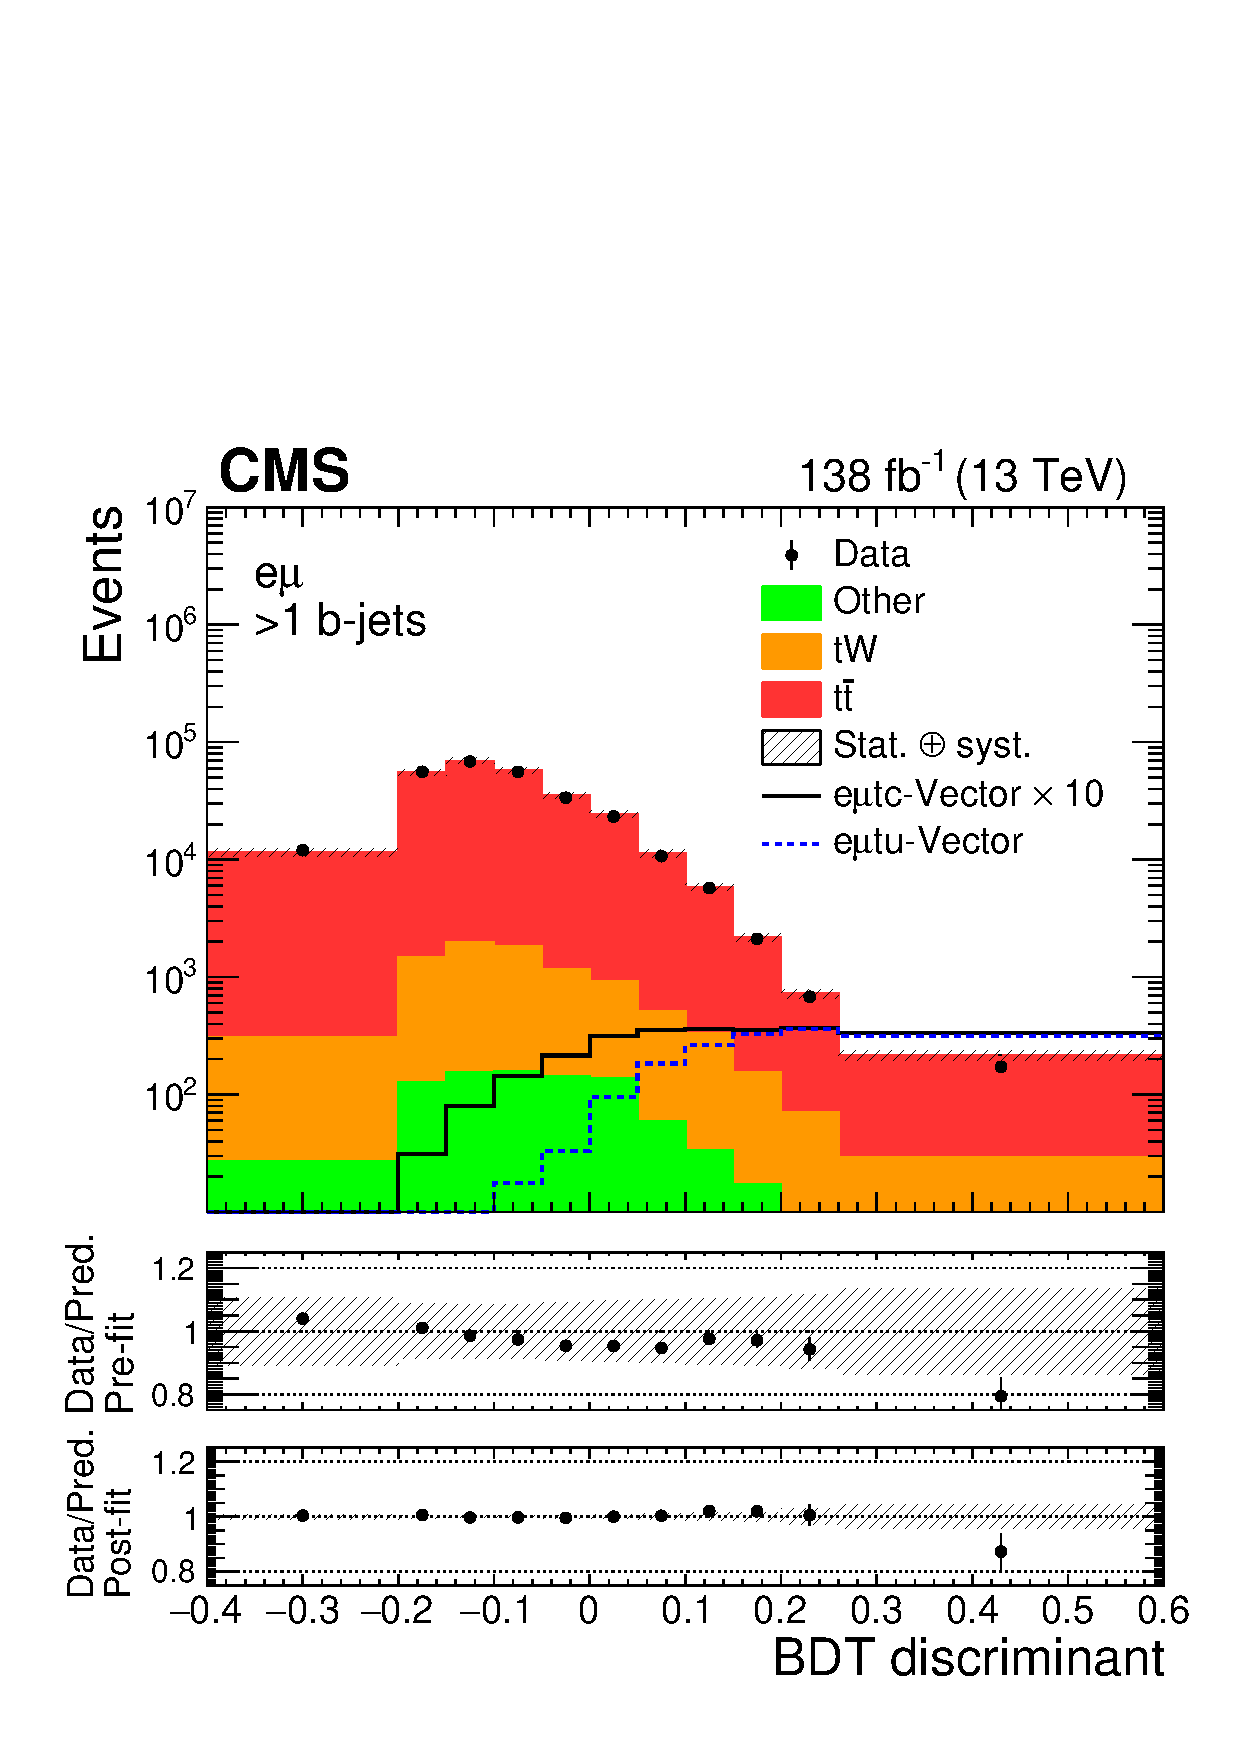
\includegraphics[width=0.48\textwidth]{figures/Part3/History/CMS_results2}\\
 \end{tabular}
 \caption{The left (right) histogram, taken from~\cite{CMS:2022ztx}, shows the distribution of the \ac{BDT} discriminator in regions with exactly (more than) one b-tagged jet. The middle (bottom) panel shows the ratio of data events and the pre-fit (post-fit) predictions.}
 \label{fig:CMS_results}
 \end{center}
\end{figure}
%%%%%%%%%%%%%%%%%%%%%%%%%%%%%%%%%%%%%%%%%%%
%%%%%%%%%%%%%%%%%%%%%%%%%%%%%%%%%%%%%%%%%%%

\section{Overview of the Present CMS Analysis}
\label{sec:CLFV_This}

This analysis searches for flavor-violating $\emut{q}$ interactions using data collected by the \ac{CMS} detector in 2016-2018, corresponding to an integrated luminosity of 138 fb$^{-1}$. The targeted final states of this analysis contain exactly three charged leptons, similar to the past \ac{ATLAS} analysis~\cite{ATLAS-CONF-2018-044}. In addition to the top quark decay signals, this analysis also considers the top quark production signals, which were first introduced by~\cite{CMS:2022ztx}. Separate \acp{SR} are defined to target these two different signals. Operators with different Lorentz structures and quark flavors are considered separately. Representative Feynman diagrams are shown in Figure~\ref{fig:CMS_FD_This}. 
 
\begin{figure}[tbh!]
 \begin{center}
 \begin{tabular}{ccc}
 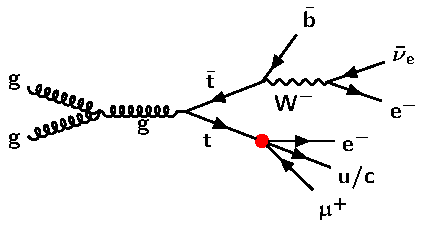
\includegraphics[width=0.31\textwidth]{figures/Part3/History/TT}&
 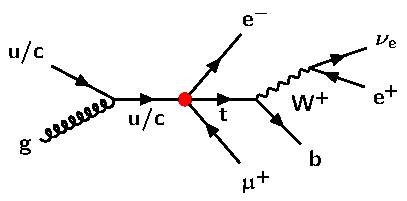
\includegraphics[width=0.33\textwidth]{figures/Part3/History/ST1}&
 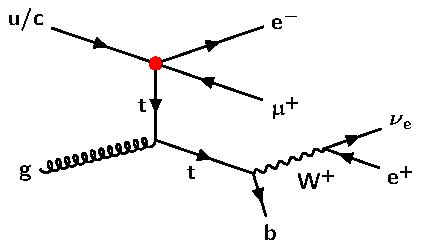
\includegraphics[width=0.31\textwidth]{figures/Part3/History/ST2}\\
 \end{tabular}
 \caption{Representative Feynman diagrams for the signal processes that are targeted by this analysis. Both top quark decay (left) and production (middle and right) \ac{CLFV} processes are shown. The top quark that does not participate in the \ac{CLFV} interaction is required to produce leptonic final states.}
 \label{fig:CMS_FD_This}
 \end{center}
 \end{figure}
 
For each \ac{SR}, one binary \ac{BDT} is trained to enhance the sensitivity of the corresponding signal mode. The \emph{nonprompt} background is estimated using a data-driven method. An upper limit at 95\% \ac{CL} is placed on the branching fraction of $\mathcal{B}(\tto{q})$ $<$ 1.2 $\times$ 10$^{-8}$, which further improves the constraint from the previous \ac{CMS}~\cite{CMS:2022ztx} by nearly a factor of 6.